\documentclass[a0paper,12pt]{article}
\usepackage[landscape,top=5cm,bottom=3cm,right=5cm,left=5cm]{geometry}
\usepackage{graphicx}
\usepackage{amsmath}
\usepackage[T1]{fontenc}
\usepackage{lmodern}
\usepackage{tikz}
\usetikzlibrary{shapes,arrows}
\usetikzlibrary{decorations.text}
\usetikzlibrary{spy,calc}
\usetikzlibrary{shapes.arrows}

\usepackage{color}
\usepackage{moresize}
\usepackage{lipsum} % dummy text
\usepackage{multicol}

\pgfdeclarelayer{background}
\pgfdeclarelayer{layer1}
\pgfdeclarelayer{layer2}
\pgfdeclarelayer{layer3}
\pgfdeclarelayer{foreground}

\newenvironment{Figure}
  {\par\medskip\noindent\minipage{\linewidth}}
  {\endminipage\par\medskip}

% This macro creates header.
\newcommand{\HEADING}[1]
{
    \includegraphics[scale=0.35]{./images/heading.png}
    \fontsize{2.5cm}{1cm}\selectfont \textcolor{red}{#1}
    \vspace{1cm}
}

\newcommand{\SECTION}[1]
{
    {\fontsize{2cm}{1.5cm}\selectfont \textsc{\textcolor{blue}{#1}}}
}

\newcommand{\CAPTION}[1]
{
    \Huge \texttt{#1}
}

\newcommand{\TEXT}[1]
{
   { \fontsize{1.5cm}{1.5cm}\fontfamily{\sfdefault}\selectfont {#1} }
}

\newcommand{\MOOSE}[0]
{
    {\TEXT{\texttt{\textcolor{red}{MOOSE}}}}
}

\tikzset{
  every overlay node/.style={
    draw=black,fill=white,rounded corners,anchor=north west,
  },
}
% Usage:
% \tikzoverlay at (-1cm,-5cm) {content};
% or
% \tikzoverlay[text width=5cm] at (-1cm,-5cm) {content};
\def\tikzoverlay{%
   \tikz[baseline,overlay]\node[draw=white,every overlay node]
}%

\begin{document}

%\begin{tikzpicture}[remember picture,overlay] 
%    \node[opacity=1.0] (background) at (current page.center) {
%    
\includegraphics[width=\paperwidth,height=\paperheight]{./background.jpg}
%};
%
%\end{tikzpicture}


\begin{minipage}{\textwidth}
    \centering
    \fontsize{4cm}{1em}\selectfont \textcolor{red}{Modelling Memory Across Scale}
    \\
    \fontsize{1.5cm}{1em}\selectfont Aditya Gilra, Aviral Goel, Dilawar Singh,
    Harsha Rani, Sahil Moza, Subhasis Ray, Upinder Bhalla
\end{minipage}



%% Three columns
\vspace{5cm}
\setlength{\columnsep}{6cm}
\begin{multicols}{3}
    
%%%%%%%%%%%% Column 1
\begin{Figure}

    \HEADING{Introduction}

    \begin{Figure}

        \begin{itemize}
            \item \TEXT{Memory and plasticity involve brain mechanisms from molecular scale
                    to enormous networks.}
            \item \TEXT{We have developed \textcolor{red}{\MOOSE}, the Multiscale Object
                    Oriented Simulation Environment, to model plasticity across scales.}
        \end{itemize}

     \begin{tikzpicture}[
        spy using outlines={circle
            , magnification=10, connect spies
        }
        , compartment/.style={cylinder
             , draw
             , cylinder uses custom fill
             , cylinder end fill = red!35
             , cylinder body fill = red!40
             , minimum height = 2cm
             , minimum width = 3cm 
         }
         , spine/.style={cylinder 
             , fill = blue!20
             , inner sep=1mm
             , minimum height=5mm
             , minimum width=10mm
         }
         , branch/.style={cylinder
             , draw
             , cylinder uses custom fill
             , cylinder end fill = red!35
             , cylinder body fill = red!40
             , minimum height = 5cm
             , minimum width = 1cm
         }
         ]
         \centering
         \node [] (image) at (0,-1) {
             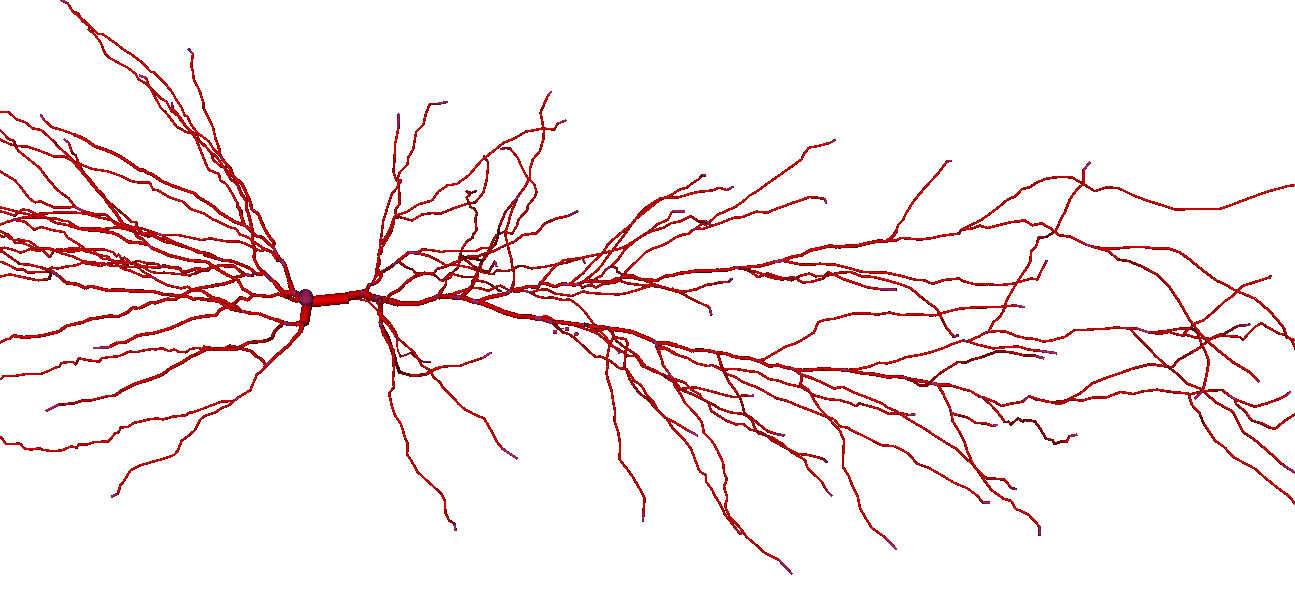
\includegraphics[scale=0.2,angle=-30]{./images/ca1_neuron.png}
         };

         \foreach \i in {-3,...,3}
         \foreach \j in {-3,...,3}
         {
             \node[fill=blue!40,opacity=0.3,thin,inner sep=0pt, minimum size=3mm,circle] (n\i\j) at (\i, \j) {};
         };

         \spy[blue, size=3cm] on (1.65, -1.5) in node[left] at (7,0);
         \node[below=4cm,text width=0.2\textwidth] {\CAPTION{Embed in network}};

         %% Cool. Now create a 3d compartment model here.
         \begin{scope}[xshift=10cm]
             \node[compartment] (c1) {};
             \node[compartment] (c2) at (c1.east) {};
             \node[compartment] (c3) at (c2.east) {};

             \node[branch,rotate=45] (b1) at ([xshift=10mm,yshift=0mm]c3.before top) {};
             \node[branch,rotate=-45] (b2) at ([xshift=5mm, yshift=-15mm]c3.base east) {};

            % Spines
            \node[spine, inner sep=1mm, rotate=135] (s11) at (b1.north east) {};
            \node[spine, inner sep=1mm, rotate=135] (s12) at ([xshift=3mm]b1.south east) {};

            \node[spine, inner sep=1mm, rotate=45] (s21) at (b2.north east) {};
            \node[spine, inner sep=1mm, rotate=45] (s22) at ([xshift=-3mm]b2.south east) {};
             
         \end{scope}

         %% Scope to draw chemisty 
         \begin{scope}

             \node[] (chemical) at ([yshift=-4cm]c2.south) {
                 \includegraphics[scale=0.2]{./images/chemical_reactions.png}
             };

             \draw[decoration={text along path, text={Chemical model}},
                 decorate] (c1.center) to [bend right] (chemical);


         \end{scope}


     \end{tikzpicture} 
     \begin{tikzpicture}
        \node[] (image) {
            \includegraphics[width=0.5\textwidth]{./images/Gallery_Moose_Multiscale.png}
        };
    \end{tikzpicture} %

    \vspace{1cm}

    \end{Figure}


    \HEADING{Multiscale Modeling in MOOSE}

    \begin{Figure}
        \centering

        \SECTION{Modular solvers available in MOOSE}

        \footnote{Write the time-scales}

        \begin{tikzpicture}
            \node[] (image) {
                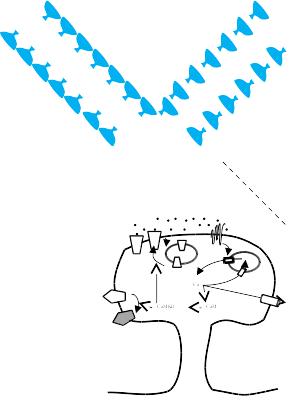
\includegraphics[width=0.15\textwidth]{./images/stochastic_solver.png}
            }; 
            \node[below=3.5cm, text width=0.3\textwidth] {\CAPTION{Stochastic(GSSA): GSolve}};
        \end{tikzpicture} \hfill
        \begin{tikzpicture}
            \node[] (image) {
                \includegraphics[width=0.15\textwidth]{./images/ksolve_dsolve.png}
            };
            \node[below=3.5cm, text width=0.3\textwidth] {\CAPTION{ODE + Diffusion: KSolve + DSolve}};
        \end{tikzpicture} \hfill
        \begin{tikzpicture}
            \node[] (image) {
                \includegraphics[width=0.15\textwidth]{./images/hsolve.png}
            };
            \node[below=3.5cm, text width=0.3\textwidth] {\CAPTION{Electrical: HSolve}};
        \end{tikzpicture}

    \end{Figure}


\end{Figure}

%% Column 2



\begin{Figure}
    \SECTION{Simulation: Putting them all-together}

    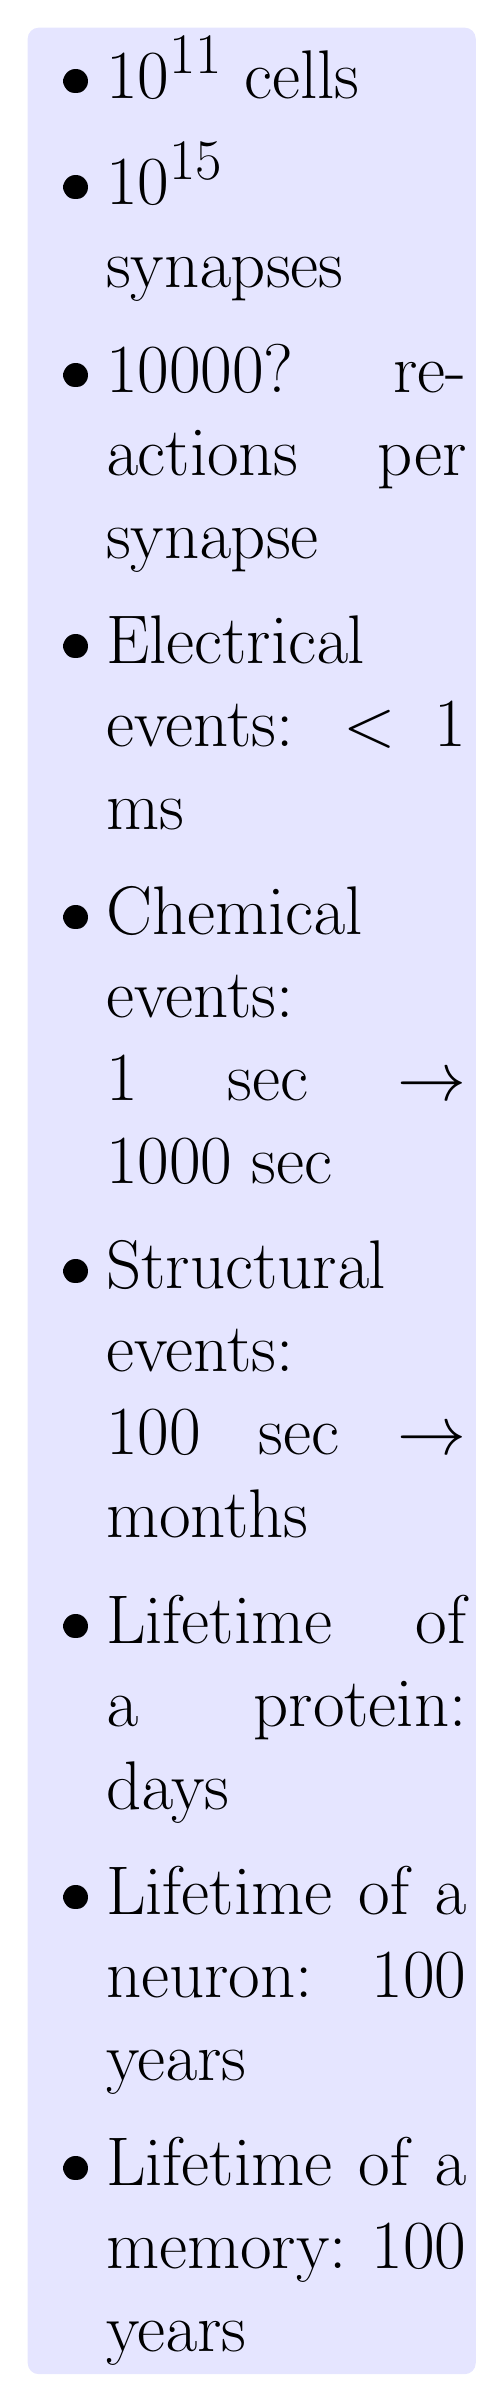
\begin{tikzpicture}
        \node[ rounded corners, fill=blue!10] (text) {
        \begin{minipage}{0.45\textwidth}
            \Huge
            \begin{itemize}
                \item $10^{11}$ cells
                \item $10^{15}$ synapses 
                \item $10000$? reactions per synapse  
                \item Electrical events: $< 1$ ms  
                \item Chemical events: $1\; \text{sec} \rightarrow 1000\; \text{sec}$ 
                \item Structural events: $100\; \text{sec} \rightarrow \text{months}$
                \item Lifetime of a protein: days 
                \item Lifetime of a neuron: 100 years 
                \item Lifetime of a memory: 100 years
            \end{itemize}

        \end{minipage}
        };
    \end{tikzpicture} %
    \begin{tikzpicture}
        \node [] (simulation) {
            \includegraphics[width=0.5\textwidth]{./images/simulation.png}
        };
    \end{tikzpicture}
\end{Figure}

\HEADING{Some projects using MOOSE}
\begin{Figure}
    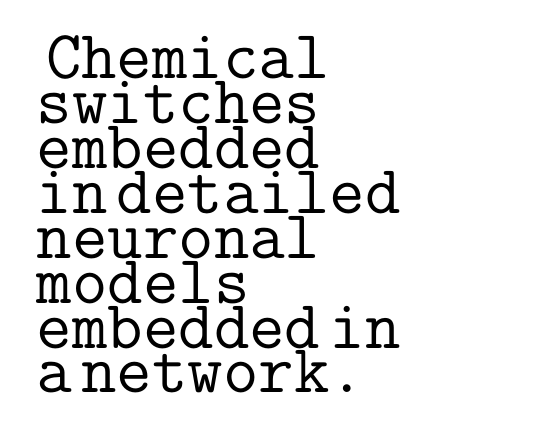
\begin{tikzpicture}

        \node[below=6cm, text width=0.5\textwidth] {\CAPTION{
                Chemical switches embedded in detailed neuronal models embedded in a
                network.}
        };

    \end{tikzpicture} %
    \begin{tikzpicture}

        \node[] (image) {
            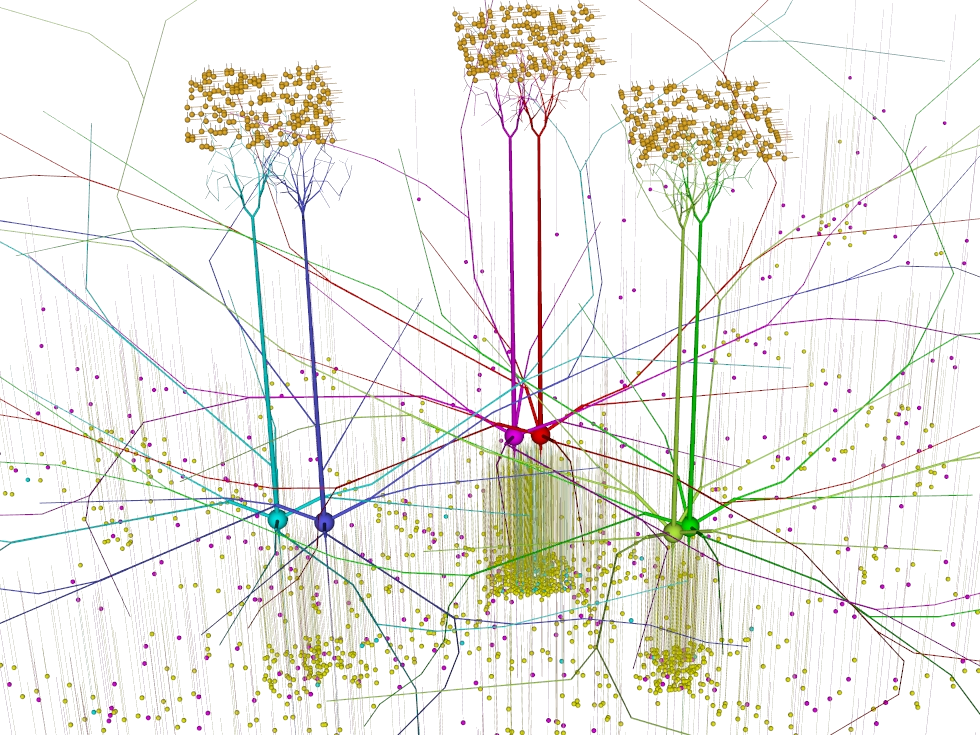
\includegraphics[width=0.5\textwidth]{./images/fullmodel_moogli.png}
        };

        \node[below=6cm,text width=0.5\textwidth]{ \CAPTION{
                Network coding and computation in olfaction and sematosensory
                cortex.}
        };

    \end{tikzpicture}%

    \begin{tikzpicture}
        \node[] (image) {
            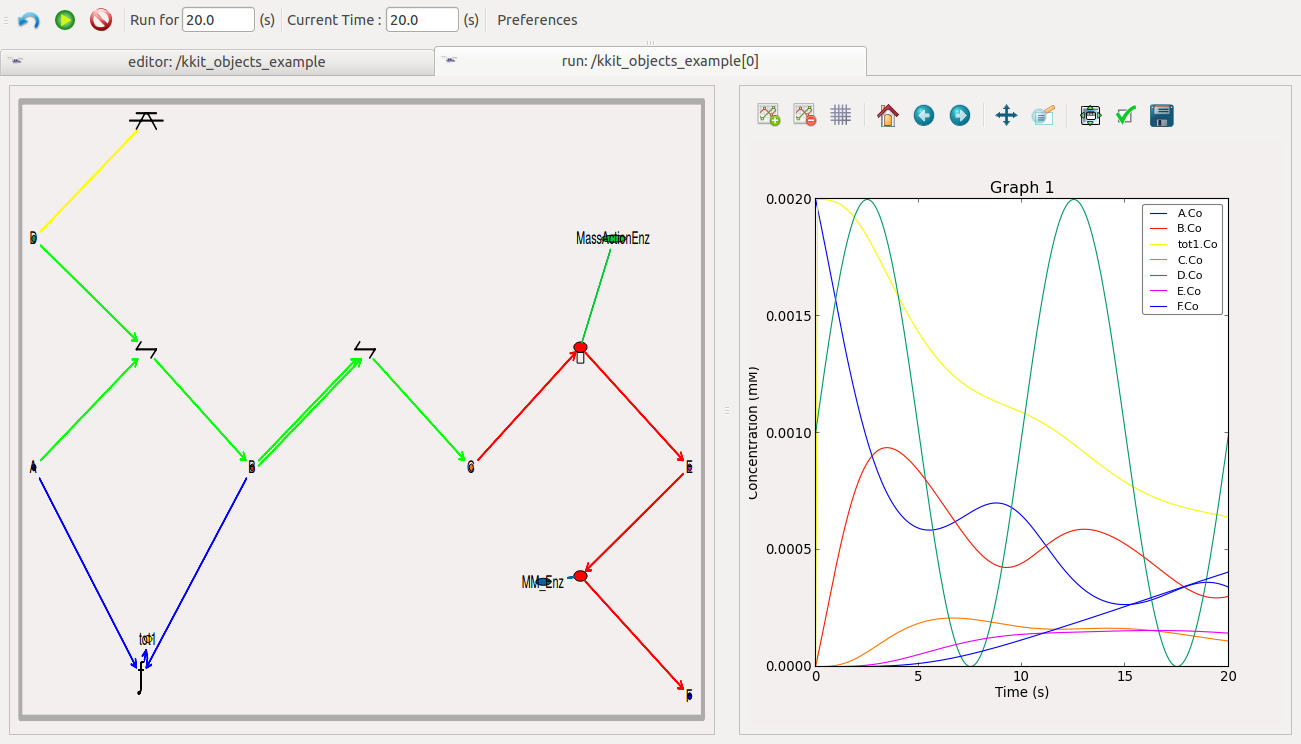
\includegraphics[width=0.5\textwidth]{./images/poster_runView.png}
        };

        \node[below=6cm,text width=0.5\textwidth] {\CAPTION{
                Robustness of chemical switches with respect to stochasticity and
                parameters.}
        };

    \end{tikzpicture}
\end{Figure}

%% Column 3
\begin{Figure}
    
    \HEADING{Summary}

    \HUGE We use models to
    \begin{itemize}
            
        \item Integrate many scales of neuronal data with basic
            physical/chemical principles.
        \item Explain phenomenon of plasticity, activity and neuronal coding.
        \item Predict circuit mechanisms, plasticity rules, and emergent
            phenomena such as \emph{decorrelation}, \emph{robustness}, and
            \emph{memory decay}.

    \end{itemize}

    \textbf{We have developed MOOSE to carry out these simulations}.

\end{Figure}

\end{multicols}

\end{document}
